\documentclass[12pt,a4paper]{article}
\usepackage[UTF8]{ctex}
\usepackage{amsmath,amssymb}
\usepackage{xcolor}
\usepackage{hyperref}
\usepackage{geometry}
\usepackage{graphicx}
\geometry{margin=2.5cm}

\title{QAOA MaxCut / QAOA MaxCut}
\author{QuoNic}
\date{}

\begin{document}
\maketitle

\begin{center}
\textbf{Algorithms / 算法} | 难度：高级 | 预计时间：20 分钟
\end{center}

\tableofcontents
\newpage

\section{为什么需要？}

QAOA MaxCut 是 QAOA 的经典应用。

\subsection{经典局限}
\begin{itemize}
  \item MaxCut 是 NP-hard 问题
  \item 经典算法只能近似求解
\end{itemize}

\subsection{量子优势}
\begin{itemize}
  \item QAOA 可以提供比经典近似算法更好的解
  \item 对噪声有鲁棒性
  \item 理论上可以达到最优解
\end{itemize}

\subsection{实际应用}
\begin{itemize}
  \item 组合优化
  \item 图论
  \item 网络设计
\end{itemize}

\section{快速上手}

\begin{verbatim}
from quonic.algorithms import qaoa_maxcut
result = qaoa_maxcut(graph=[(0,1),(1,2),(2,0)], p=2)
print(f'MaxCut: {result.maxcut_value}')
\end{verbatim}

\textbf{预期输出}：
\begin{verbatim}
MaxCut: 2
\end{verbatim}

\section{原理详解}

\subsection{电路图}

\begin{center}
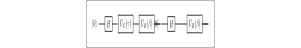
\includegraphics[width=0.6\textwidth]{../../images/qaoa_maxcut_circuit.svg}
\end{center}

\subsection{数学推导}

QAOA MaxCut 优化：
\begin{equation}
C(z) = \sum_{(i,j) \in E} w_{ij} (1 - z_i z_j)
\end{equation}

\textbf{QAOA 电路}：
\begin{equation}
|\gamma, \beta\rangle = \prod_{l=1}^{p} e^{-i\beta_l B} e^{-i\gamma_l C} |+\rangle^{\otimes n}
\end{equation}

\subsection{几何解释}

QAOA MaxCut 在参数空间中寻找最优割。

\section{代码详解}

\begin{verbatim}
from quonic.algorithms import qaoa_maxcut

# qaoa_maxcut(graph, p, optimizer)
# graph: list of edges (i, j)
# p: number of QAOA layers
# optimizer: classical optimizer
result = qaoa_maxcut(graph=[(0,1),(1,2),(2,0)], p=2)
print(f'MaxCut: {result.maxcut_value}')
\end{verbatim}

\section{进阶用法}

\subsection{场景 1：不同层数}

\begin{verbatim}
from quonic.algorithms import qaoa_maxcut
for p in [1, 2, 4]:
    result = qaoa_maxcut(graph=[(0,1),(1,2),(2,0)], p=p)
    print(f'p={p}: MaxCut={result.maxcut_value}')
\end{verbatim}

\section{适用场景}

\subsection{组合优化}

QAOA MaxCut 可以用于各种组合优化问题。

\subsection{图论}

QAOA MaxCut 可以用于图分割问题。

\section{常见问题}

\subsection{QAOA MaxCut 的近似比是多少？}

对于 MaxCut，QAOA 的近似比约为 0.692。

\subsection{QAOA MaxCut 需要多少层？}

层数 $p$ 越大，近似比越好。

\section{学习路径}

\subsection{前置知识}
\begin{itemize}
  \item QAOA
  \item 组合优化
  \item 图论
\end{itemize}

\subsection{继续学习}
\begin{itemize}
  \item 图着色
  \item 旅行商问题
  \item 量子优化
\end{itemize}

\section{完整示例代码}

\subsection{示例 1：基本 QAOA MaxCut}

\begin{verbatim}
from quonic.algorithms import qaoa_maxcut
result = qaoa_maxcut(graph=[(0,1),(1,2),(2,0)], p=2)
print(f'MaxCut: {result.maxcut_value}')
\end{verbatim}

\section{下载}

\begin{itemize}
  \item [qaoa\_maxcut.py](https://github.com/ChrisLee0721/QuoNic/blob/main/examples/qaoa_maxcut/qaoa_maxcut.py)
\end{itemize}

\end{document}
